\subsection{VDCU(Vehicle Dynamics Control Unit)}
VDCU is a vehicle dynamics control unit. It manipulates torque request from driver pedal to calculate final torque for all 4 motors. The calculated torque never exceed driver request as driver request is processed as torque limitation Traction control can only decrease the total amount of requested torque.

\subsubsection{Description}
Board uses only LV and 2x CAN bus.\\
HW :\\
-Texas Instruments C2000 Delfino F28377 MCU\\
-5V can transceiver TJA1049\\

\noindent SW:\\
Board is programmed using simulink embedded coder. Advantage is that we can use our developed code for IPG Carmaker simulation (MIL) directly into our formula. VDCU uses pedal position, inertial measurement, steering wheel sensor, wheel speed sensor and motor encoders to manipulate the torque. Measurements are fed into our yaw rate control system. Output is a torque vector fed to torque vectoring algorithm that calculates the torque distribution for all wheels The resultant torque for individual wheels is lowered by traction control algorithm if needed and fed to motors.

\begin{figure}[H]
	\centering
	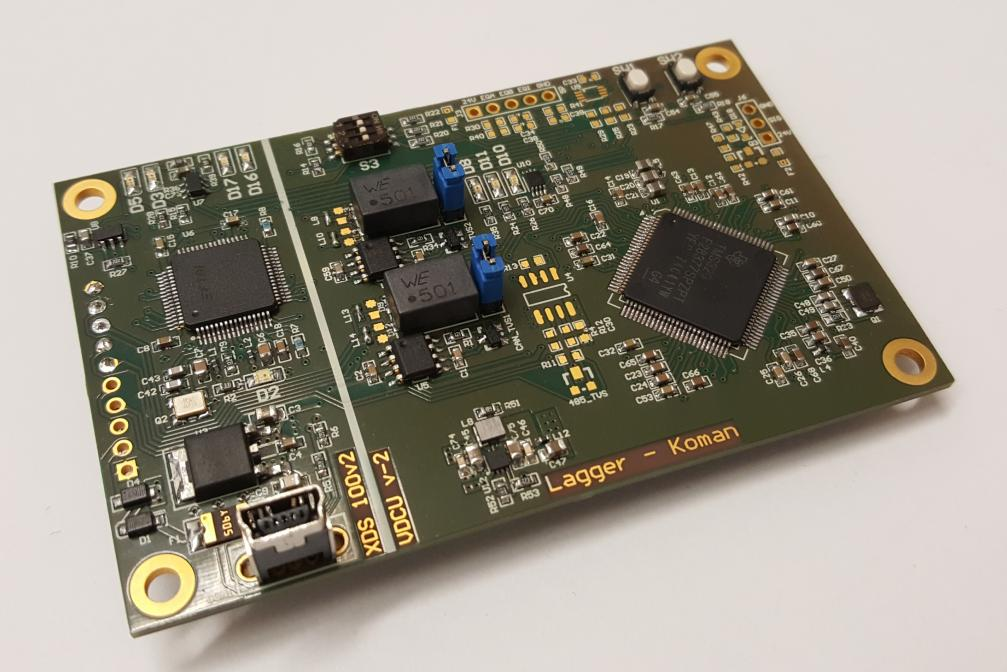
\includegraphics[width=\textwidth]{./img/VDCU-pcb.jpg}
	\caption{PCB of VDCU.}
	\label{fig:VDCU-pcb}
\end{figure}

\subsubsection{Wiring, cables}
Module is connected using headers to ECUB.

\subsubsection{Position in car}
Inside ECUB box.

\subsection{LV part 2}
Describe those parts here which interfere or influence the tractive system, for example a controlling unit that measures wheel speeds and steering angle and calculates a target torque for each motor or a DC/DC-Converter providing power for the LV-system from the HV-system, etc.

\subsubsection{Description}
Describe the parts used and their circuitry, and provide main operation parameters, use tables or figures, etc.

\subsubsection{Wiring, cables}
Describe the wiring, show schematics, etc.

\subsubsection{Position in car}
Provide CAD-renderings showing the relevant parts. Mark the parts in the rendering, if necessary.